\section{Design Option Structuring} \label{ch:design}
This chapter gives an overview of initial design concept selection, focusing on the different missions aspects of configuration, mission profile and control mechanisms. This concept generation is done systematically by means of a \acrfull{dot} for each of the aspects. Combination of the different trees then yields a number of final concepts. The next phase is eliminating clearly unfeasible or undevelopable concepts. The first section gives a \gls{dot} for each of the mission aspects in subsequent subsections, including eliminating unfeasible options. The second section proposes the generation of concepts used in the next phase of concept selection and trade-off, to take place after the \gls{br}.

%\subsection{Deceleration mechanism}
%Deceleration can be performed by purely aerodynamic forces exerted by the local atmosphere, as used in the \gls{irve} missions (see Table \ref{tab:hiadcomparison}), primarily by a propulsive force (retro-propulsion) or a hybrid configuration featuring both, as used in for example the Apollo entry vehicles. Aerodynamic deceleration reduces the $\Delta V$ required by propulsion and is hence preferable to propulsive deceleration, i.e. retro-propulsion, through a decrease of the required entry mass by limiting required propellant to be taken on board. A feasibility study of \gls{nasa} indicates that pure propulsion is unfeasible by the large amounts of propellant mass required \cite{Cianciolo2010}. Moreover, by means of Tsiolkovsky's rocket equation it can be shown that a velocity increment of 7 $[km/s]$ is unattainable while keeping deceleration mechanism mass below 10 percent of initial mass for conventional effective exhaust velocities \cite{Wertz2011}. Figure \ref{fig:dotdelmech} gives the \gls{dot} for the deceleration mechanism.
%
%Other options are un(der)developed: studies on their application for (re-)entry have not been found nor have these been considered in feasibility studies by \gls{nasa}, predominantly the extensive studies of Cianciolo et al \cite{Cianciolo2010}. As such, while these options may be worth revisiting in the future, their current state of development does not allow for implementation in a (re-)entry vehicle.
%
%\begin{figure}[H]
%\centering
%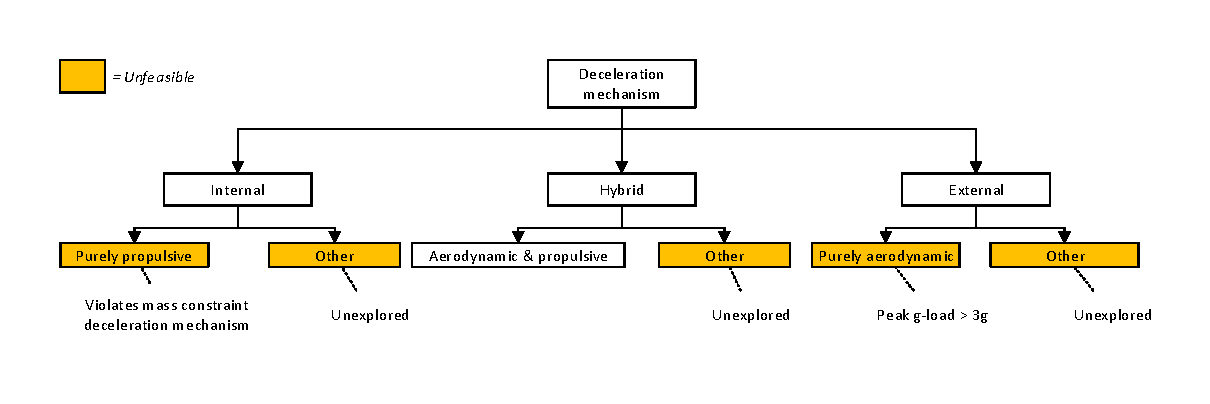
\includegraphics[width = 0.85\textwidth]{Figure/DOT_decelerationmechanism.pdf}
%\caption{Design Option Tree for entry vehicle deceleration mechanism}
%\label{fig:dotdelmech}
%\end{figure}
\subsection{Design Option Trees}
This section presents the \gls{dot}s for the three aspects of vehicle configuration, mission profile and control mechanisms. These are combined in the next step of concept generation to yield a number of concepts for further selection and analysis, as described in the next section.
\subsubsection{Configuration of aerodynamic deceleration}
The configuration of the aerodynamic deceleration mechanism, given in figure \ref{fig:dotconfig}, can be at a first level be subdivided into inflatable and non-inflatable systems. For non-inflatable systems an \textit{AND} subdivision can be made. A blunt or pointed body can be considered and at the same time this structure may be deployable or undependable. Pointed bodies will not be considered since the attached shock will cause excessive aerodynamic heating \cite{AndersonJr.2007} making this concept unfeasible. The blunt body may further be subdivided into lifting and non-lifting bodies. Lifting bodies is a body that produces lift by itself, i.e. does not need to be placed at an angle of attack. Non-lifting-bodies, or ballistic bodies, may feature a lifting component by featuring a \gls{cg} located away from the symmetry axis. This \gls{cg} offset is sometimes also actively used for control purposes\cite{Dillman2012} as is also explained in section \ref{sec:DOTcontrol}. 

The second separation is  the subdivision between deployable and non-deployable structures. Where as for inflatable structures deployment is inherent to the design non-inflatable structure may feature no deployment mechanism. The deployable configurations feature a change in geometry specifically for the reentry which can for example be controlled by actuators. The deployable systems are already cut off due to the more complicated (thus less reliable) deployment combined with the inherent higher weight of non-inflatable structures \cite{Cianciolo2010} compared to deployable inflatables.

The inflatable structures on the right hand side of Figure \ref{fig:dotconfig} can be subdivided in fore or aft placed inflatables or a combination thereof. This can be further broken down to an Isotensoid, tension cone and stacked configuration. Variations here off are also examined by \gls{nasa}\cite{Smith2010}. A Isotensoid configuration consists of a single inflatable covering the whole frontal surface area. In a tension cone structural rigidity is provided by only a single inflatable outer ring, which is filled in between with fabric. Finally a stacked configuration features simply multiple inflatables which are stacked to form the desired configuration.

The inflatable structures on the right hand side of Figure \ref{fig:dotconfig} can be subdivided in fore or aft placed inflatables or a combination thereof. Attached inflatables can be further broken down to an isotensoid, tension cone and stacked configuration. An isotensoid configuration consists of a single inflatable covering the whole frontal surface area. In a tension cone structural rigidity is provided by only a single inflatable outer ring, which is filled in between with fabric. Finally a stacked configuration features multiple inflatables which are stacked to form the desired configuration. \cite{Smith2011, Yamada2009, Hughes2005} Trailing inflatables are derivatives of the Disk-Gap-Band parachute concept and, as their name suggests, trail the payload capsule \cite{Smith2010}. The feasibility of a such a ballute has been investigated and a ballute is deemed feasible and effective in terms of mass for aerocapture, albeit not specifically aimed at Mars entry \cite{Rohrschneider2007, Miller2003}.

\begin{figure}[H]
%\centering
\hspace{-23mm}
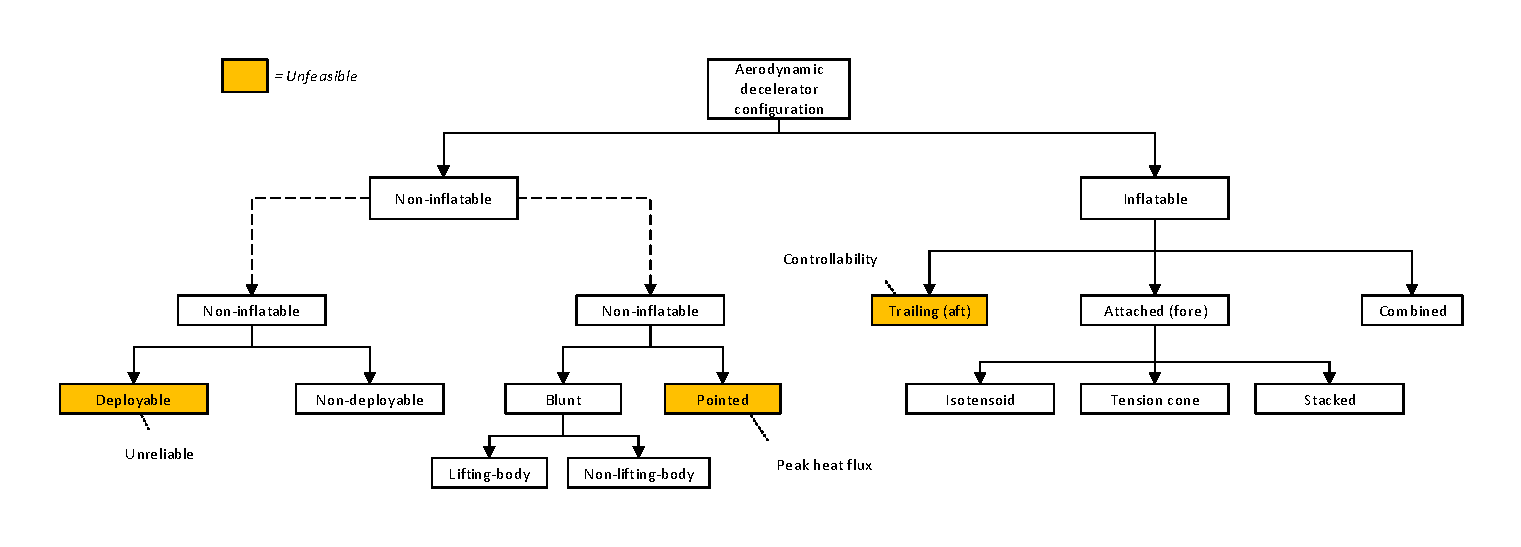
\includegraphics[width = 1.25\textwidth]{Figure/DOT_configuration.pdf}
\vspace{-5mm}
\caption{Design Option Tree for entry vehicle configuration}
\label{fig:dotconfig}
\end{figure}

%\subsection{Design Considerations}
%\subsubsection{Deceleration mechanism}
%Deceleration can be performed by purely aerodynamic forces exerted by the local atmosphere, as used in the \gls{irve} missions (see Table \ref{tab:hiadcomparison}), primarily by a propulsive force (retro-propulsion) or a hybrid configuration featuring both, as used in for example the Apollo entry vehicles. Aerodynamic deceleration reduces the $\Delta V$ required by propulsion and is hence preferable to propulsive deceleration, i.e. retro-propulsion, through a decrease of the required entry mass by limiting required propellant to be taken on board. A feasibility study of \gls{nasa} indicates that pure propulsion is unfeasible by the large amounts of propellant mass required \cite{Cianciolo2010}. Moreover, by means of Tsiolkovsky's rocket equation it can be shown that a velocity increment of 7 $[km/s]$ is unattainable while keeping deceleration mechanism mass below 10 percent of initial mass for conventional effective exhaust velocities \cite{Wertz2011}. Figure \ref{fig:dotdelmech} gives the \gls{dot} for the deceleration mechanism.

%Other options are un(der)developed: studies on their application for (re-)entry have not been found nor have these been considered in feasibility studies by \gls{nasa}, predominantly the extensive studies of Cianciolo et al \cite{Cianciolo2010}. As such, while these options may be worth revisiting in the future, their current state of development does not allow for implementation in a (re-)entry vehicle.

%\begin{figure}[H]
%\centering
%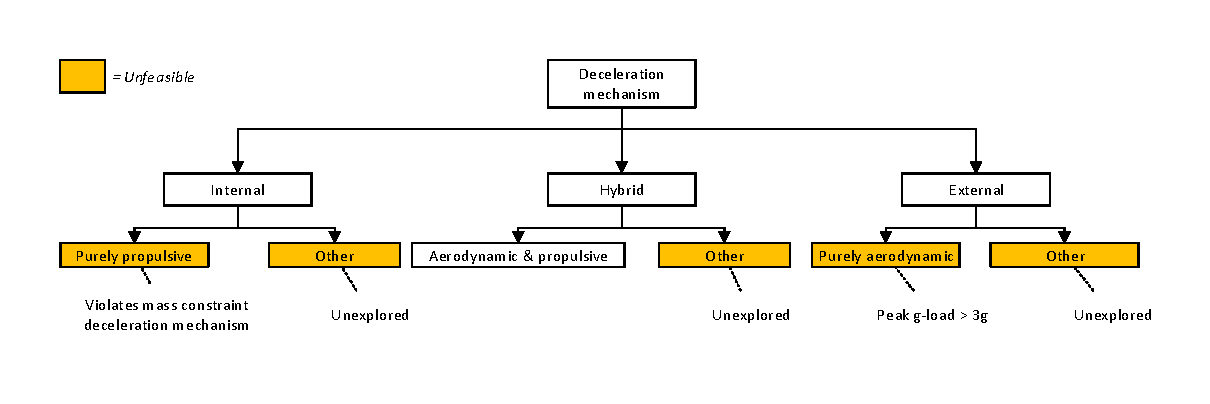
\includegraphics[width = 0.85\textwidth]{Figure/DOT_decelerationmechanism.pdf}
%\caption{Design Option Tree for entry vehicle deceleration mechanism}
%\label{fig:dotdelmech}
%\end{figure}

\subsubsection{Mission profile} \label{sec:DOTprofile}
In terms of mission profile, freedom exists in the rate at which kinetic energy is dissipated. On one hand a short mission duration can be used, in the order of minutes or hours, featuring a steep descent; on the other hand a longer mission duration can be used, in the order of days or weeks (or longer), featuring a shallow descent. The rate at which kinetic energy, conforming to a velocity of 7 km/s, is dissipated places a lower bound on the mission duration. Entry in the order of minutes becomes prohibitive for the thermal and mechanical loads, which will most likely be in excess of the 3g limit imposed (requirement CIA-A07).  An upper bound is placed by the requirement (CIA-A08) that aerobraking duration shall be less than ten (Earth) days. In a first estimation one can therefore distinguish mission profiles in the order of hours on one hand and days on the other hand. 
\begin{figure}[H]
\centering
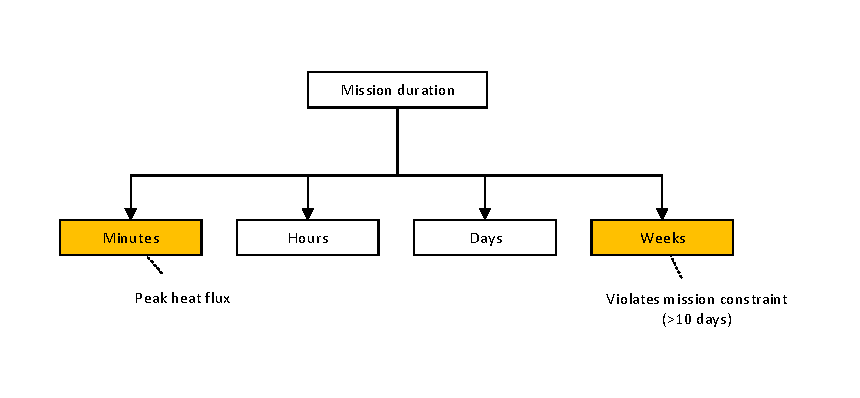
\includegraphics[width = 1.0\textwidth]{Figure/DOT_missionduration.pdf}
\vspace{-5mm}
\caption{Design Option Tree for entry vehicle configuration}
\label{fig:dotconfig}
\end{figure}

\subsubsection{Control} \label{sec:DOTcontrol}
\begin{figure}[H]
\centering
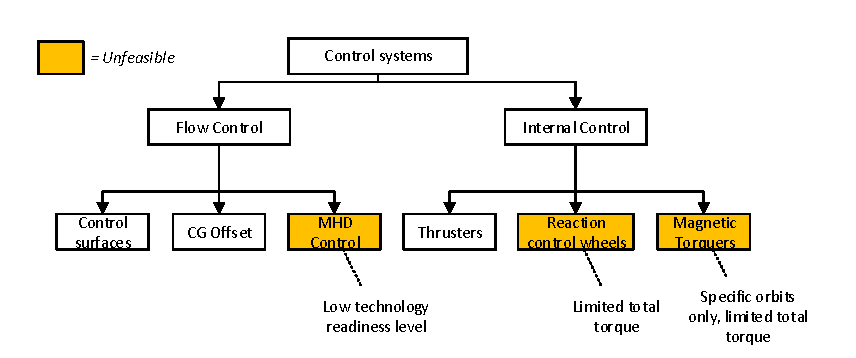
\includegraphics[width = 0.93\textwidth]{Figure/DOT_control.pdf}
\vspace{-5mm}
\caption{Design Option Tree for control systems}
\label{fig:dotconfig}
\end{figure}
Control options are classified as either flow control or internal control. The former uses means to deflect the aerodynamic flow around the vehicle to create a reaction force. In terms of internal control, the only feasible option is the use of thrusters. Reaction control wheels are deemed infeasible by the limited total torque they can deliver, unable to deliver the torques required to change the attitude of the (re-)entry vehicle while keeping within mass constraints \cite{Wertz2011}. Magnetic torquers are limited by the fact that these only function in certain orbits and are moreover limited in the total torque they can deliver \cite{Wertz2011}. Thrusters, however, are a feasible option in terms of internal control. In terms of flow control, control by \gls{mhd} is deemed unfeasible by the fact that it is a relatively new technology and thereby at a low level of technology readiness \cite{Braun2009}. As such, it inherently has a lower level of reliability, in conflict with requirement CIA-B01-01-04-Contr-01. Control surfaces change the shape of the entry vehicle and thereby its interaction with the flow, while a \gls{cg} offset changes the inclination of the body in the flow. This concept was succesfully introduced in the \gls{irve3} concept \cite{Dillman2012}.


%\subsection{Inflation system}
%As mentioned in Chapter \ref{cha:litreview}, inflation can be performed either with (ram-air) or without use of the atmosphere. A third option is the use of both (hybrid), thereby featuring ram-air inlets as well as internal gas storage and feed systems. In terms of the medium used for inflation, conventionally nitrogen gas is used. An alternative would be hydrazine gas, as explained in Chapter \ref{cha:litreview}.

\subsection{Concept generation}
This section presents a proposed strategy for the generation and selection of concepts based on the \gls{dot}s given in the previous section. The \gls{dot}s presented previously form the basis for concept selection: the feasible end-nodes of the trees are combined to yield a number of concepts. For example one of these combinations would be a rigid lifting body with long mission duration and control via aerodynamic shape alteration. From this number of concepts the unfeasible combinations are firstly eliminated. This is followed upon by eliminating the weakest concepts. The remaining concepts are then used for further analysis, to yield a select number of concepts deemed most viable to fulfill the mission need statement, as stated in Ref.\cite{Balasooriyan2015}. After formulation of a set of trade-off criteria, the concepts are then analyzed for their performance in terms of these criteria. A review of this process takes place in the \gls{mtr}. A trade-off then yields the concept selected for further analysis and design, with the \gls{fr} as final activity.